\begin{figure}[!t]
	\centering
	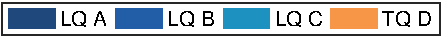
\includegraphics[width=0.6\linewidth]{fig/b3_example_legend}
	\\
	\subfloat[DRF cannot provide LQs with performance guarantee. ]{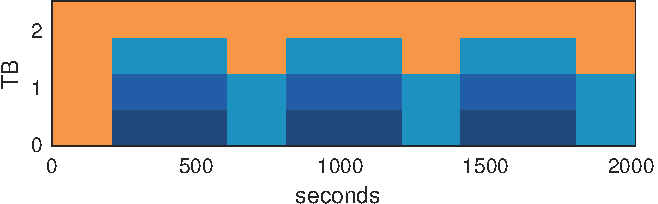
\includegraphics[width=0.8\linewidth]{fig/b3_example_DRF}\label{fig:example-DRF}}
	\\
	\subfloat[Strict Priority (SP) starves the TQ and cannot gurantee performance for conflicting LQs .]{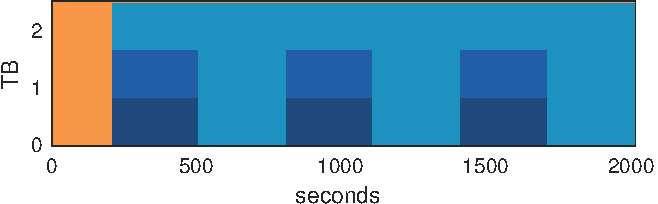
\includegraphics[width=0.8\linewidth]{fig/b3_example_SP}\label{fig:example-Strict}}
	\\
	\subfloat[(DRF + SP) serves one of LQs by SP and leaves the rest to DRF. It is not the bad solution but is there any better one?]{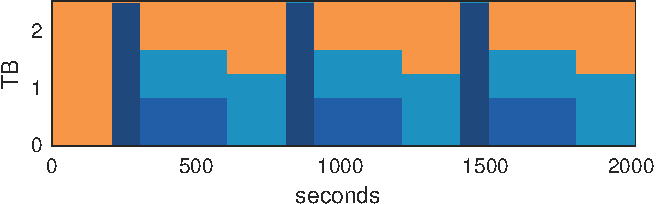
\includegraphics[width=0.8\linewidth]{fig/b3_example_SimpleBestRejectAll}\label{fig:example-simple}}	
	\\
	\subfloat[Optimal solution prioritizes as many queues as possible without hurting other queues. ]{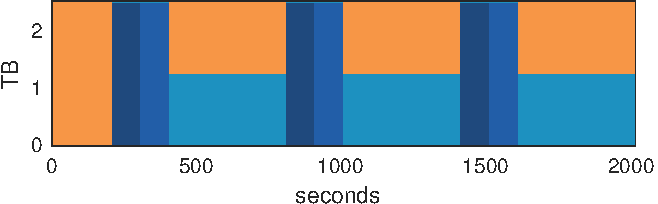
\includegraphics[width=0.8\linewidth]{fig/b3_example_BPF}\label{fig:example-optimum}}	
	\caption{}
	\label{fig:example}
\end{figure}